% Options for packages loaded elsewhere
\PassOptionsToPackage{unicode}{hyperref}
\PassOptionsToPackage{hyphens}{url}
%
\documentclass[
]{article}
\usepackage{lmodern}
\usepackage{amsmath}
\usepackage{ifxetex,ifluatex}
\ifnum 0\ifxetex 1\fi\ifluatex 1\fi=0 % if pdftex
  \usepackage[T1]{fontenc}
  \usepackage[utf8]{inputenc}
  \usepackage{textcomp} % provide euro and other symbols
  \usepackage{amssymb}
\else % if luatex or xetex
  \usepackage{unicode-math}
  \defaultfontfeatures{Scale=MatchLowercase}
  \defaultfontfeatures[\rmfamily]{Ligatures=TeX,Scale=1}
\fi
% Use upquote if available, for straight quotes in verbatim environments
\IfFileExists{upquote.sty}{\usepackage{upquote}}{}
\IfFileExists{microtype.sty}{% use microtype if available
  \usepackage[]{microtype}
  \UseMicrotypeSet[protrusion]{basicmath} % disable protrusion for tt fonts
}{}
\makeatletter
\@ifundefined{KOMAClassName}{% if non-KOMA class
  \IfFileExists{parskip.sty}{%
    \usepackage{parskip}
  }{% else
    \setlength{\parindent}{0pt}
    \setlength{\parskip}{6pt plus 2pt minus 1pt}}
}{% if KOMA class
  \KOMAoptions{parskip=half}}
\makeatother
\usepackage{xcolor}
\IfFileExists{xurl.sty}{\usepackage{xurl}}{} % add URL line breaks if available
\IfFileExists{bookmark.sty}{\usepackage{bookmark}}{\usepackage{hyperref}}
\hypersetup{
  hidelinks,
  pdfcreator={LaTeX via pandoc}}
\urlstyle{same} % disable monospaced font for URLs
\usepackage[margin=1in]{geometry}
\usepackage{color}
\usepackage{fancyvrb}
\newcommand{\VerbBar}{|}
\newcommand{\VERB}{\Verb[commandchars=\\\{\}]}
\DefineVerbatimEnvironment{Highlighting}{Verbatim}{commandchars=\\\{\}}
% Add ',fontsize=\small' for more characters per line
\usepackage{framed}
\definecolor{shadecolor}{RGB}{248,248,248}
\newenvironment{Shaded}{\begin{snugshade}}{\end{snugshade}}
\newcommand{\AlertTok}[1]{\textcolor[rgb]{0.94,0.16,0.16}{#1}}
\newcommand{\AnnotationTok}[1]{\textcolor[rgb]{0.56,0.35,0.01}{\textbf{\textit{#1}}}}
\newcommand{\AttributeTok}[1]{\textcolor[rgb]{0.77,0.63,0.00}{#1}}
\newcommand{\BaseNTok}[1]{\textcolor[rgb]{0.00,0.00,0.81}{#1}}
\newcommand{\BuiltInTok}[1]{#1}
\newcommand{\CharTok}[1]{\textcolor[rgb]{0.31,0.60,0.02}{#1}}
\newcommand{\CommentTok}[1]{\textcolor[rgb]{0.56,0.35,0.01}{\textit{#1}}}
\newcommand{\CommentVarTok}[1]{\textcolor[rgb]{0.56,0.35,0.01}{\textbf{\textit{#1}}}}
\newcommand{\ConstantTok}[1]{\textcolor[rgb]{0.00,0.00,0.00}{#1}}
\newcommand{\ControlFlowTok}[1]{\textcolor[rgb]{0.13,0.29,0.53}{\textbf{#1}}}
\newcommand{\DataTypeTok}[1]{\textcolor[rgb]{0.13,0.29,0.53}{#1}}
\newcommand{\DecValTok}[1]{\textcolor[rgb]{0.00,0.00,0.81}{#1}}
\newcommand{\DocumentationTok}[1]{\textcolor[rgb]{0.56,0.35,0.01}{\textbf{\textit{#1}}}}
\newcommand{\ErrorTok}[1]{\textcolor[rgb]{0.64,0.00,0.00}{\textbf{#1}}}
\newcommand{\ExtensionTok}[1]{#1}
\newcommand{\FloatTok}[1]{\textcolor[rgb]{0.00,0.00,0.81}{#1}}
\newcommand{\FunctionTok}[1]{\textcolor[rgb]{0.00,0.00,0.00}{#1}}
\newcommand{\ImportTok}[1]{#1}
\newcommand{\InformationTok}[1]{\textcolor[rgb]{0.56,0.35,0.01}{\textbf{\textit{#1}}}}
\newcommand{\KeywordTok}[1]{\textcolor[rgb]{0.13,0.29,0.53}{\textbf{#1}}}
\newcommand{\NormalTok}[1]{#1}
\newcommand{\OperatorTok}[1]{\textcolor[rgb]{0.81,0.36,0.00}{\textbf{#1}}}
\newcommand{\OtherTok}[1]{\textcolor[rgb]{0.56,0.35,0.01}{#1}}
\newcommand{\PreprocessorTok}[1]{\textcolor[rgb]{0.56,0.35,0.01}{\textit{#1}}}
\newcommand{\RegionMarkerTok}[1]{#1}
\newcommand{\SpecialCharTok}[1]{\textcolor[rgb]{0.00,0.00,0.00}{#1}}
\newcommand{\SpecialStringTok}[1]{\textcolor[rgb]{0.31,0.60,0.02}{#1}}
\newcommand{\StringTok}[1]{\textcolor[rgb]{0.31,0.60,0.02}{#1}}
\newcommand{\VariableTok}[1]{\textcolor[rgb]{0.00,0.00,0.00}{#1}}
\newcommand{\VerbatimStringTok}[1]{\textcolor[rgb]{0.31,0.60,0.02}{#1}}
\newcommand{\WarningTok}[1]{\textcolor[rgb]{0.56,0.35,0.01}{\textbf{\textit{#1}}}}
\usepackage{graphicx}
\makeatletter
\def\maxwidth{\ifdim\Gin@nat@width>\linewidth\linewidth\else\Gin@nat@width\fi}
\def\maxheight{\ifdim\Gin@nat@height>\textheight\textheight\else\Gin@nat@height\fi}
\makeatother
% Scale images if necessary, so that they will not overflow the page
% margins by default, and it is still possible to overwrite the defaults
% using explicit options in \includegraphics[width, height, ...]{}
\setkeys{Gin}{width=\maxwidth,height=\maxheight,keepaspectratio}
% Set default figure placement to htbp
\makeatletter
\def\fps@figure{htbp}
\makeatother
\setlength{\emergencystretch}{3em} % prevent overfull lines
\providecommand{\tightlist}{%
  \setlength{\itemsep}{0pt}\setlength{\parskip}{0pt}}
\setcounter{secnumdepth}{-\maxdimen} % remove section numbering
\ifluatex
  \usepackage{selnolig}  % disable illegal ligatures
\fi

\author{}
\date{\vspace{-2.5em}}

\begin{document}

\startappendices

\hypertarget{appendix}{%
\section{Appendix}\label{appendix}}

\hypertarget{conditional-distributions}{%
\paragraph{Alternative distributions than the
normal}\label{conditional-distributions}}

Student's t-distribution

\noindent A common alternative for the normal distribution is the
Student t distribution. Similarly to the normal distribution, it is also
symmetric (skewness is equal to zero if \(\nu > 3\)). The probability
density function (pdf), consistent with @ghalanos2020, is given by
equation @ref(eq:stdghalanos). As will be seen in @ref(vol-mod), GARCH
models are used for volatility modeling in practice. @bollerslev1987
examined the use of the GARCH-Student or GARCH-t model as an alternative
to the standard Normal distribution, which relaxes the assumption of
conditional normality by assuming the standardized innovation to follow
a standardized Student t-distribution {[}@bollerslev2008{]}.

\begin{align}
f(x; \alpha, \beta,\nu) = \dfrac{\Gamma(\dfrac{\nu+1}{2})}{\Gamma(\dfrac{\nu}{2})\sqrt{\beta \pi \nu}} \left(1+\dfrac{(x-\alpha)^2}{\beta \nu}\right)^{-(\nu+1)/2}
 (\#eq:stdghalanos)
\end{align}

\noindent where \(\alpha, \beta\) and \(\nu\) are respectively the
location, scale and shape (tail-thickness) parameters. \(\nu/2\) is
equal to the \(q\)\footnote{Also referred to as \(n\) by
  @theodossiou1998 or \(\eta\) by @bali2008} parameter (which we call
\(\eta\)) of the SGT distribution. The symbol \(\Gamma\) is the Gamma
function.

\noindent Unlike the normal distribution, which depends entirely on two
moments only, the student t distribution allows for fatter tails. This
kurtosis coefficient is given by equation @ref(eq:kurt) if \(\nu>4\).
This is useful while as already mentioned, the standardized residuals
appear to have fatter tails than the normal distribution following
@bollerslev2008.

\begin{align}
kurt = 3 + \dfrac{6}{\nu-4}
 (\#eq:kurt)
\end{align}

Generalized Error Distribution

\noindent The GED distribution is nested in the generalized t
distribution by @mcdonald1988 is used in the GED-GARCH model by
@nelson1991 to model stock market returns. This model replaced the
assumption of conditional normally distributed error terms by
standardized innovations that following a generalized error
distribution. It is a symmetric, uni-modal distribution (location
parameter is the mode, median and mean). This is also sometimes called
the exponential power distribution {[}@bollerslev2008{]}. The
conditional density (pdf) is given by equation @ref(eq:ged) following
@ghalanos2020.

\begin{align}
f(x; \alpha, \beta, \kappa) = \dfrac{\kappa e^{-\frac{1}{2}\left|\dfrac{x-\alpha}{\beta}\right|^\kappa}}{2^{1+1/\kappa}\beta\Gamma(1/\kappa)}
 (\#eq:ged)
\end{align}

where \(\alpha, \beta\) and \(\kappa\) are respectively the location,
scale and shape parameters.

Skewed t-distribution

\noindent The density function can be derived following @fernández1998
who showed how to introduce skewness into uni-modal standardized
distributions {[}@trottier2015{]}. The first equation from
@trottier2015, here equation @ref(eq:skeweddist) presents the skewed
t-distribution.

\begin{align}
f_{\xi}(z) \equiv \frac{2 \sigma_{\xi}}{\xi+\xi^{-1}} f_{1}\left(z_{\xi}\right), \quad z_{\xi} \equiv\left\{\begin{array}{ll}
\xi^{-1}\left(\sigma_{\xi} z+\mu_{\xi}\right) & \text { if } z \geq-\mu_{\xi} / \sigma_{\xi} \\
\xi\left(\sigma_{\xi} z+\mu_{\xi}\right) & \text { if } z<-\mu_{\xi} / \sigma_{\xi}
\end{array}\right.
 (\#eq:skeweddist)
\end{align}

\noindent where
\(\mu_{\xi} \equiv M_{1}\left(\xi-\xi^{-1}\right), \quad \sigma_{\xi}^{2} \equiv\left(1-M_{1}^{2}\right)\left(\xi^{2}+\xi^{-2}\right)+2 M_{1}^{2}-1, \quad M_{1} \equiv 2 \int_{0}^{\infty} u f_{1}(u) d u\)
and \(\xi\) between \(0\) and \(\infty\). \(f_1(\cdot)\) is in this case
equation @ref(eq:stdghalanos), the pdf of the student t distribution
coming to equation @ref(eq:stdist), which has the parameterization
following the SGT parameters.

\begin{equation}
\begin{array}{c}f_{S T}(x ; \alpha, \beta, \xi, \eta)=\frac{\Gamma\left(\frac{1}{2}+\eta\right)}{\sqrt{\beta\pi \eta} \Gamma(\eta)\left(\frac{|x-\alpha+m|^{2}}{\eta\beta(\xi \operatorname{sign}(x-\alpha+m)+1)^{2}}+1\right)^{\frac{1}{2}+\eta}} \\m=\frac{2 \xi \sqrt{\beta\eta} \Gamma\left(\eta-\frac{1}{2}\right)}{\sqrt{\pi} \Gamma\left(\eta+\frac{1}{2}\right)}\end{array}
 (\#eq:stdist)
\end{equation}

\noindent According to @giot2003; @giot2004, the skewed t-distribution
outperforms the symmetric density distributions.

Skewed Generalized Error Distribution

\noindent What also will be interesting to examine is the SGED
distribution of @theodossiou2000 in GARCH models, as in the work of
@lee2008. The SGED distribution extends the Generalized Error
Distribution (GED) to allow for skewness and leptokurtosis. The density
function can be derived following @fernández1998 who showed how to
introduce skewness into uni-modal standardized distributions
{[}@trottier2015{]}. It can also be found in @theodossiou2000. The pdf
is then given by the same equation @ref(eq:skeweddist) as the skewed
t-distribution but with \(f_1(\cdot)\) equal to equation @ref(eq:ged).
To then get equation @ref(eq:sged).

\begin{equation}
\begin{array}{c}
f_{S G E D}(x ; \alpha, \beta, \xi, \kappa)=\frac{\kappa e^{-\left(\frac{|x-\alpha+m|}{\nu \beta(1+\xi \operatorname{sig}(x-\alpha+m))}\right)^{p}}}{2 \nu \beta \Gamma(1 / p)} \\
m=\frac{2^{\frac{2}{p}} \nu \beta \xi \Gamma\left(\frac{1}{2}+\frac{1}{p}\right)}{\sqrt{\pi}}
\end{array}
(\#eq:sged)
\end{equation}

\(f_{S G E D}(x ; \alpha, \beta, \xi, p)=\frac{p e^{-\left(\frac{|x-\alpha+m|}{\nu \beta(1+\xi \operatorname{sig}(x-\alpha+m))}\right)^{p}}}{2 \nu \beta \Gamma(1 / p)} \\m=\frac{2^{\frac{2}{p}} \nu \beta \xi \Gamma\left(\frac{1}{2}+\frac{1}{p}\right)}{\sqrt{\pi}}\)

SGT (Skewed Generalized t-distribution)

\noindent The SGT distribution of introduced by @theodossiou1998 and
applied by @bali2007 and @bali2008. According to @bali2008 the proposed
solutions (use of historical simulation, student's t-distribution,
generalized error distribution or a mixture of two normal distributions)
to the non-normality of standardized financial returns only partially
solved the issues of skewness and leptokurtosis. The density of the
generalized t-distribution of @mcdonald1988 can be rewritten as its skew
variant following @trottier2015. The pdf of the SGT distribition is
given by eqution @ref(eq:sgt).

\begin{equation}
\begin{array}{c}
f_{S G T}(x ; \alpha, \beta, \xi, \kappa, \eta)=\frac{\kappa}{2 v \beta \eta^{1 / \kappa} B\left(\frac{1}{\kappa}, \eta\right)\left(\frac{|x-\alpha +m|^{\kappa}}{\eta(v \beta)^{\kappa}(\xi \operatorname{sign}(x-\alpha+m)+1)^{\kappa}}+1\right)^{\frac{1}{\kappa}+\eta}} \\
m=\frac{2 v \beta \xi \eta^{\frac{1}{\kappa}} B\left(\frac{2}{\kappa}, \eta-\frac{1}{\kappa}\right)}{B\left(\frac{1}{\kappa}, \eta\right)}
\end{array}
(\#eq:sgt)
\end{equation}

\noindent Following @theodossiou1998 however, there are two parameters,
\(\kappa\)\footnote{Referred to as \(\kappa\) by @theodossiou1998 and
  @bali2008, but \(p\) by Carter Davis in the ``sgt'' package.}and
\(\eta\)\footnote{Also referred to as \(n\) by @theodossiou1998 or
  \(\eta\) by @bali2008. This is the \(q\) by Carter Davis in the
  ``sgt'' packages.}) for the shape in the SGT distribution. The \(p\)
is the peakedness parameter. The \(q\) is the tail-thickness parameter.
It is equal to the degrees of freedom \(\eta\) divided by 2 if
\(\xi = 0\) and \(\kappa = 2\), there is referred to symbol \(\nu\) in
the tables (although this is not fully statistically correct to
interprete this like degrees of freedom at all times). As shown in the
following figure @ref(fig:figure) adapted by Carter Davis using , from
the SGT the other distributions in the figure are limiting cases of the
SGT.

\begin{figure}

{\centering 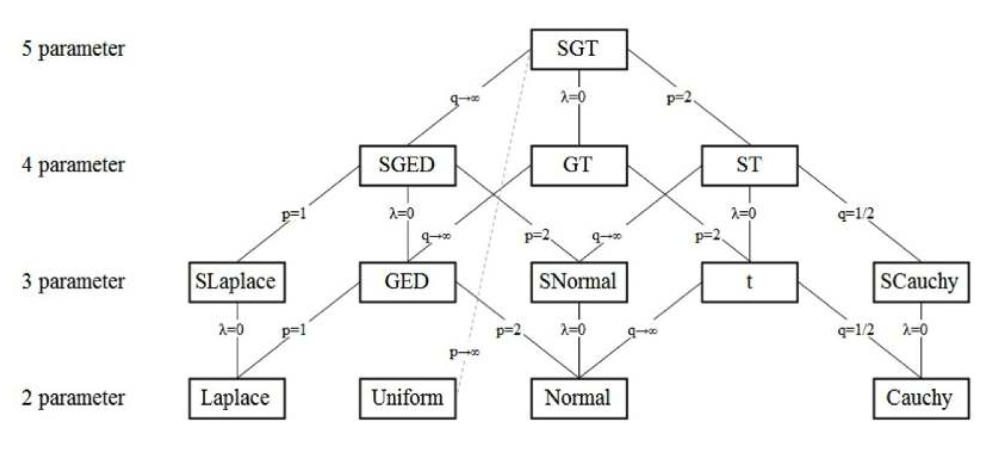
\includegraphics[width=1\linewidth]{SGT} 

}

\caption{Source: https://cran.r-project.org/web/packages/sgt}\label{fig:figure}
\end{figure}

\hypertarget{garch-models}{%
\paragraph{GARCH models}\label{garch-models}}

All the GARCH models are estimated using the package ``rugarch'' by
@alexios2020. We use specifications similar to @ghalanos2020. Parameters
have to be restricted so that the variance output always is positive,
except for the EGARCH model, as this model does not mathematically allow
for a negative output.

Symmetric (normal) GARCH model

\noindent The standard GARCH model {[}@bollerslev1986{]} is written
consistent with @ghalanos2020 as in equation @ref(eq:eq13) without
external regressors.

\begin{align}
\sigma_t^2 = \omega  + \sum\limits_{j = 1}^q {{\alpha_j}\varepsilon _{t-j}^2 +} \sum\limits_{j=1}^p {{\beta_j}\sigma_{t-j}^2} 
 (\#eq:eq13)
\end{align}

\(\sigma_t^2 = \omega + \sum\limits_{j = 1}^q {{\alpha_j}\varepsilon _{t-j}^2 +} \sum\limits_{j=1}^p {{\beta_j}\sigma_{t-j}^2}\)

\noindent where \(\sigma_t^2\) denotes the conditional variance,
\(\omega\) the intercept and \(\varepsilon_t^2\) the residuals from the
used mean process. The GARCH order is defined by \((q, p)\) (ARCH,
GARCH). As @ghalanos2020 describes: "one of the key features of the
observed behavior of financial data which GARCH models capture is
volatility clustering which may be quantified in the persistence
parameter \(\hat{P}\) specified as in equation @ref(eq:eq14).

\begin{align}
\hat{P} = \sum\limits_{j = 1}^q {{\alpha_j}}  + \sum\limits_{j = 1}^p {{\beta_j}}.
 (\#eq:eq14)
\end{align}

\noindent The unconditional variance of the standard GARCH model of
Bollerslev is very similar to the ARCH model, but with the Garch
parameters (\(\beta\)'s) included as in equation @ref(eq:eq15).

\begin{equation}
\begin{split}
\hat{\sigma}^2 
&= \dfrac{\hat{\omega}}{1 - \hat{P}} \\
&= \dfrac{\hat{\omega}}{1 - \alpha - \beta}
\end{split}
 (\#eq:eq15)
\end{equation}

IGARCH model

\noindent Following @ghalanos2020, the integrated GARCH model
{[}@bollerslev1986{]} can also be estimated. This model assumes the
persistence \(\hat{P} = 1\). This is done by Ghalanos, by setting the
sum of the ARCH and GARCH parameters to 1. Because of this
unit-persistence, the unconditional variance cannot be calculated.

GJRGARCH model

\noindent The GJRGARCH model {[}@glosten1993{]}, which is an alternative
for the asymmetric GARCH (AGARCH) by @engle1990 and @engle1993, models
both positive as negative shocks on the conditional variance
asymmetrically by using an indicator variable \(I_t-j\), it is specified
as in equation @ref(eq:eq17).

\begin{align}
\sigma_t^2 = \omega + \sum\limits_{j=1}^q (\alpha_j \varepsilon_{t-j}^2 + \gamma_j I_{t-j} \varepsilon_{t-j}^2) + \sum\limits_{j = 1}^p \beta_j \sigma_{t-j}^2
 (\#eq:eq17)
\end{align}

\noindent where \(\gamma_j\) represents the \emph{leverage} term. The
indicator function \(I\) takes on value 1 for \(\varepsilon \le 0\), 0
otherwise. Because of the indicator function, persistence of the model
now crucially depends on the asymmetry of the conditional distribution
used according to @ghalanos2020.

EGARCH model

\noindent The EGARCH model or exponential GARCH model {[}@nelson1991{]}
is defined as in equation @ref(eq:eq16). The advantage of the EGARCH
model is that there are no parameter restrictions, since the output is
log variance (which cannot be negative mathematically), instead of
variance.

\begin{align}
\log_e(\sigma_t^2) = \omega + \sum\limits_{j=1}^q (\alpha_j z_{t-j} + \gamma_j (|z_{t-j}| - E|z_{t-j}|))+ \sum\limits_{j = 1}^p \beta_j \log_e(\sigma_{t-j}^2)
 (\#eq:eq16)
\end{align}

\noindent where \(\alpha_j\) captures the sign effect and \(\gamma_j\)
the size effect.

NAGARCH model

\noindent The NAGARCH or nonlinear asymmetric model {[}@engle1993{]}. It
is specified as in equation @ref(eq:eq18). The model is
\emph{asymmetric} as it allows for positive and negative shocks to
differently affect conditional variance and \emph{nonlinear} because a
large shock is not a linear transformation of a small shock.

\begin{align}
\sigma_t^2 = \omega + \sum\limits_{j=1}^q \alpha_j (\varepsilon_{t-j}+ \gamma_j \sqrt{\sigma_{t-j}})^2 + \sum\limits_{j = 1}^p \beta_j \sigma_{t-j}^2
 (\#eq:eq18)
\end{align}

\(\sigma_t^2 = \omega + \sum\limits_{j=1}^q \alpha_j (\varepsilon_{t-j}+ \gamma_j \sqrt{\sigma_{t-j}})^2 + \sum\limits_{j = 1}^p \beta_j \sigma_{t-j}^2\)

As before, \(\gamma_j\) represents the \emph{leverage} term.

TGARCH model

\noindent The TGarch or threshold model {[}@zakoian1994{]} also models
assymetries in volatility depending on the sign of the shock, but
contrary to the GJRGARCH model it uses the conditional standard
deviation instead of conditional variance. It is specified as in
@ref(eq:eq19).

\begin{align}
\sigma_t = \omega + \sum\limits_{j=1}^q (\alpha_j^+ \varepsilon_{t-j}^+ \alpha_j^{-} + \varepsilon_{t-j}^{-}) + \sum\limits_{j = 1}^p \beta_j \sigma_{t-j}
 (\#eq:eq19)
\end{align}

\noindent where \(\varepsilon_{t-j}^+\) is equal to
\(\varepsilon_{t-j}\) if the term is negative and equal to 0 if the term
is positive. The reverse applies to \(\varepsilon_{t-j}^-\). They cite
@davidian1987 who find that using volatility instead of variance as
scaling input variable gives better variance estimates. This is due to
absolute residuals (contrary to squared residuals with variance) more
closely predicting variance for non-normal distributions.

TSGARCH model

\noindent The absolute value Garch model or TS-Garch model, as named
after @taylor1986 and @schwert1989, models the conditional standard
deviation and is intuitively specified like a normal GARCH model, but
with the absolute value of the shock term. It is specified as in
@ref(eq:eq20).

\begin{align}
\sigma_t = \omega + \sum\limits_{j=1}^q (\alpha_j \left|\varepsilon_{t-j}\right|) +
\sum\limits_{j = 1}^p \beta_j \sigma_{t-j}
 (\#eq:eq20)
\end{align}

\newpage

\(\sigma_t = \omega + \sum\limits_{j=1}^q (\alpha_j \left|\varepsilon_{t-j}\right|) +\sum\limits_{j = 1}^p \beta_j \sigma_{t-j}\)

EWMA

\noindent A alternative to the series of GARCH models is the
exponentially weighted moving average or EWMA model. This model
calculates conditional variance based on the shocks from previous
periods. The idea is that by including a smoothing parameter \(\lambda\)
more weight is assigned to recent periods than distant periods. The
\(\lambda\) must be less than 1. It is specified as in @ref(eq:eq21).

\begin{align}
\sigma_t^2 = (1-\lambda) \sum\limits_{j=1}^\infty (\lambda^j \varepsilon_{t-j}^2)
 (\#eq:eq21)
\end{align}

In practice a \(\lambda\) of 0.94 is often used, such as by the
financial risk management company RiskMetrics\(^{TM}\) model of J.P.
Morgan {[}@morganguarantytrustcompany1996{]}.

\newpage

\hypertarget{goodness-of-fit}{%
\paragraph{Goodness of fit}\label{goodness-of-fit}}

As already mentioned, next to testing the models in part @ref(analysis),
we also tested other models using the different distributions. This we
did in order to check if distributions that capture the higher moment
effects are really better in terms of goodness of fit. We did a small
data mining experiment with 248 models that were estimated. This can
ofcourse lead to overfitting if we from this list of models select the
one with the lowest AIC for example. However, we can decide if there is
a trend using the different distributions for the several GARCH models.
Thus, in this experiment, our rule of thumb was to examine general
trends. As you can see in figure @ref(fig:aic1)

\begin{Shaded}
\begin{Highlighting}[]
\NormalTok{knitr}\SpecialCharTok{::}\FunctionTok{include\_graphics}\NormalTok{(}\StringTok{"symmetric aics.pdf"}\NormalTok{)}
\end{Highlighting}
\end{Shaded}

\begin{figure}

{\centering 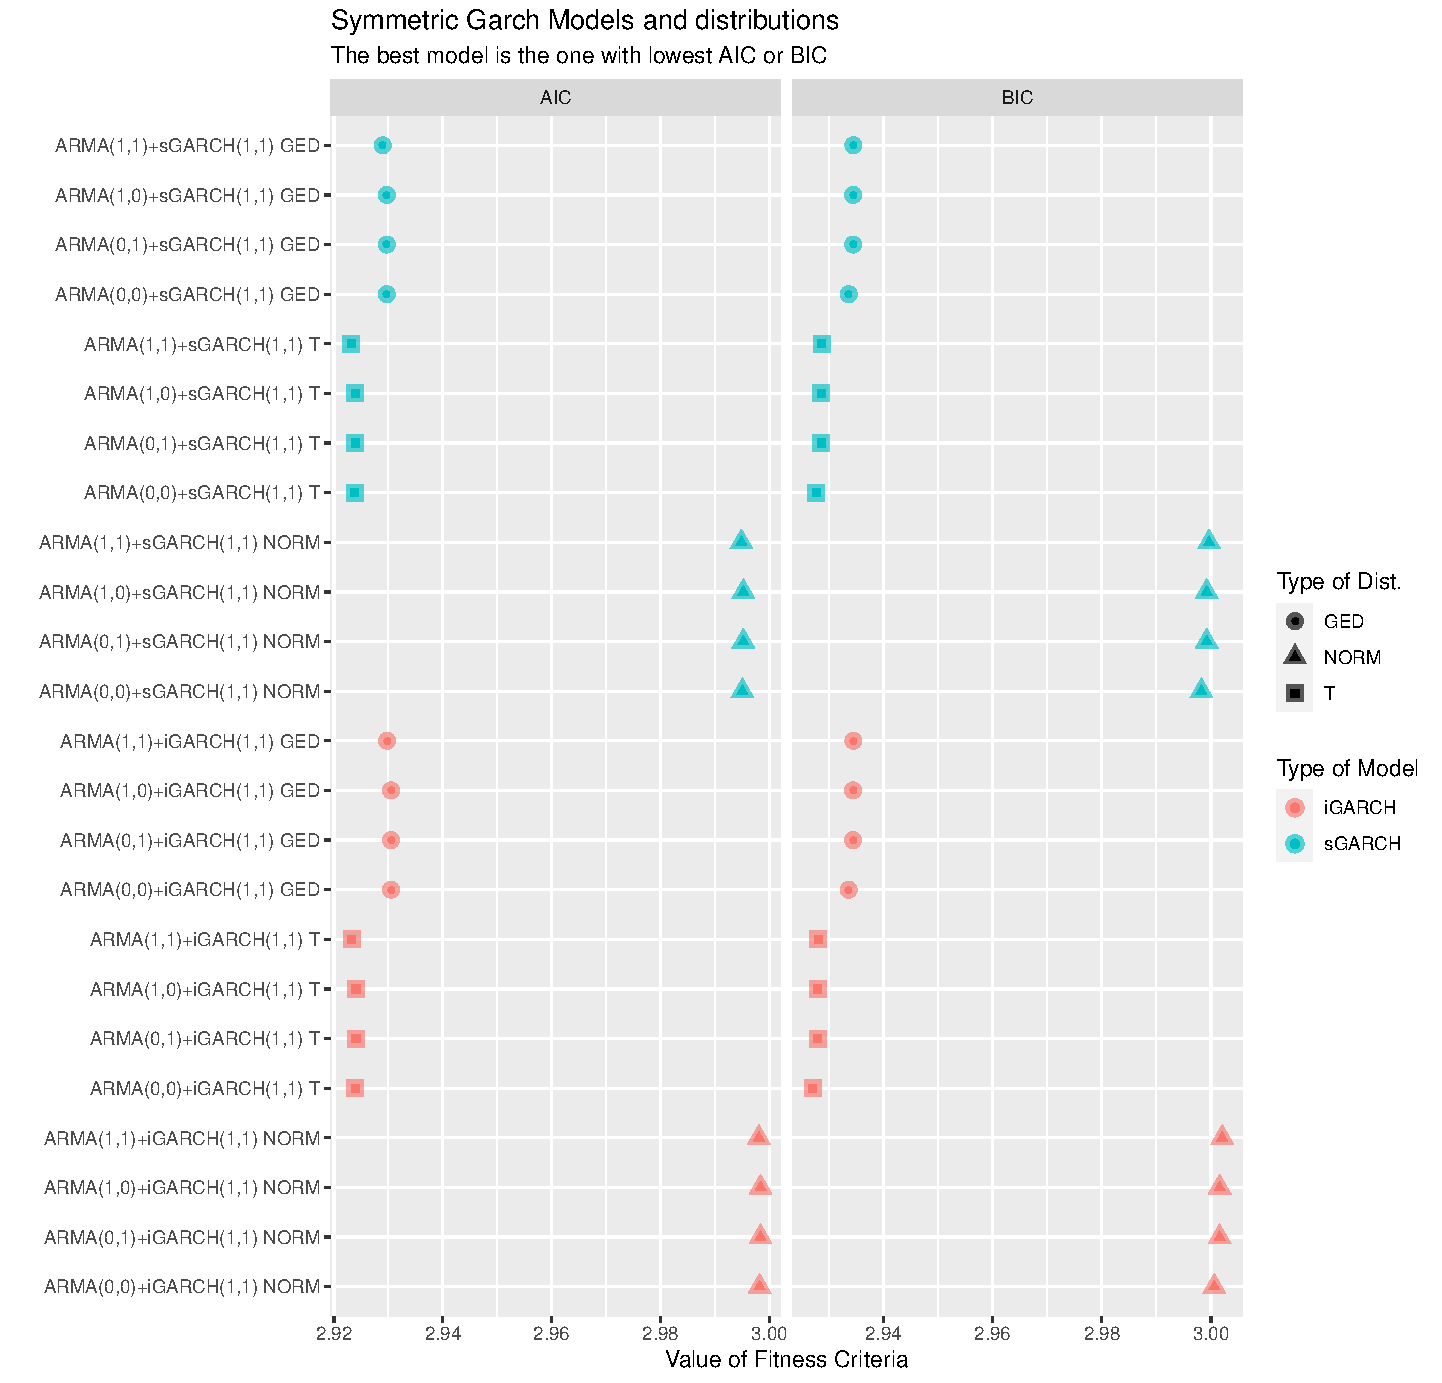
\includegraphics[width=1\linewidth]{symmetric aics} 

}

\caption{Goodness of fit symmetric GARCH and distributions}\label{fig:aic1}
\end{figure}

\end{document}
